 \documentclass[9pt]{beamer}
 \usepackage{pdfpages}
%\documentclass[compress,9pt,usenames,dvipsnames]{beamer}
% \usepackage[utf8]{inputenc}
% \includeonlyframes{current}
\input{Common-White}
% If you have a file called "university-logo-filename.xxx", where xxx
% is a graphic format that can be processed by latex or pdflatex,
% resp., then you can add a logo as follows:

% \pgfdeclareimage[height=1cm]{Emory}{figs/Emory.png}


\title % (optional, use only with long paper titles)
{
  Nicholas Eisenberg's Oral Exam
}

% \subtitle
% {Research Plan} % (optional)

\author{ \small
  Thesis committee:\\[1em]
  \small Le Chen\\[0.5em]
 \small Erkan Nane\\[0.5em]
 \small Jerzy Szugla\\[0.5em]
 \small Xiaoying Han\\[0.5em]
 \small Jimmy Hilliard\\[3em]
  {\small Parker Hall 328}\\[1em]
  {\small 2:00pm -- 4:00pm, July 24, 2022}
}


% \institute[Auburn University]{
%  \textcolor{gray}{Github Hash:~\gitAbbrevHash} \\[1em]
%  \textcolor{gray}{\gitCommitterIsoDate} \\[1em]
%  {\tiny\textcolor{gray}{\url{https://github.com/chenle02/2012_Science_Summer_Institute_Auburn_Probability_by_Le}}}
%  \vspace{5em}
% }

\date[Auburn]{
  Auburn University
}




\begin{document}
\begin{frame}[noframenumbering] \titlepage
\end{frame}
\begin{frame}[fragile,t] % publications
\begin{enumerate}
  \item Le Chen and Nicholas Eisenberg.\\
  \item[] Interpolating the stochastic heat and wave equations with time-independent noise:
    solvability and exact asymptotics.
  \item[] {\it Stochastic Partial Differential Equations: Analysis and Computation}.
  \item[] In press, 2022.
     \vfill
  \item Le Chen and Nicholas Eisenberg.\\
  \item[] Invariant measures for the nonlinear stochastic heat equation with no drift term.
  \item[] In preparation.
     \vfill
  \item Le Chen, Nicholas Eisenberg, Erkan Nane, and Alex Negash.\\
  \item[] Global solutions for the interpolated stochastic heat and wave equations with a super-linear diffusion term.
  \item[] In preparation.
\end{enumerate}
\end{frame}
\begin{frame}[fragile,t] % Timeline
\begin{center}
  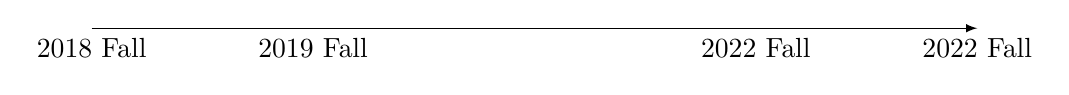
\begin{tikzpicture}[scale=1, transform shape, x=8em]
    \tikzset{>=latex}
    \draw [->] (0,0) node [below] {2018 Fall} --
      (1,0) node [below] {2019 Fall} --
      (3,0) node [below] {2022 Fall} --
      (4,0) node [below] {2022 Fall};
  \end{tikzpicture}
\end{center}
\end{frame}
\begin{frame}{Ancestral Shrine} % Shrine
\begin{center}
  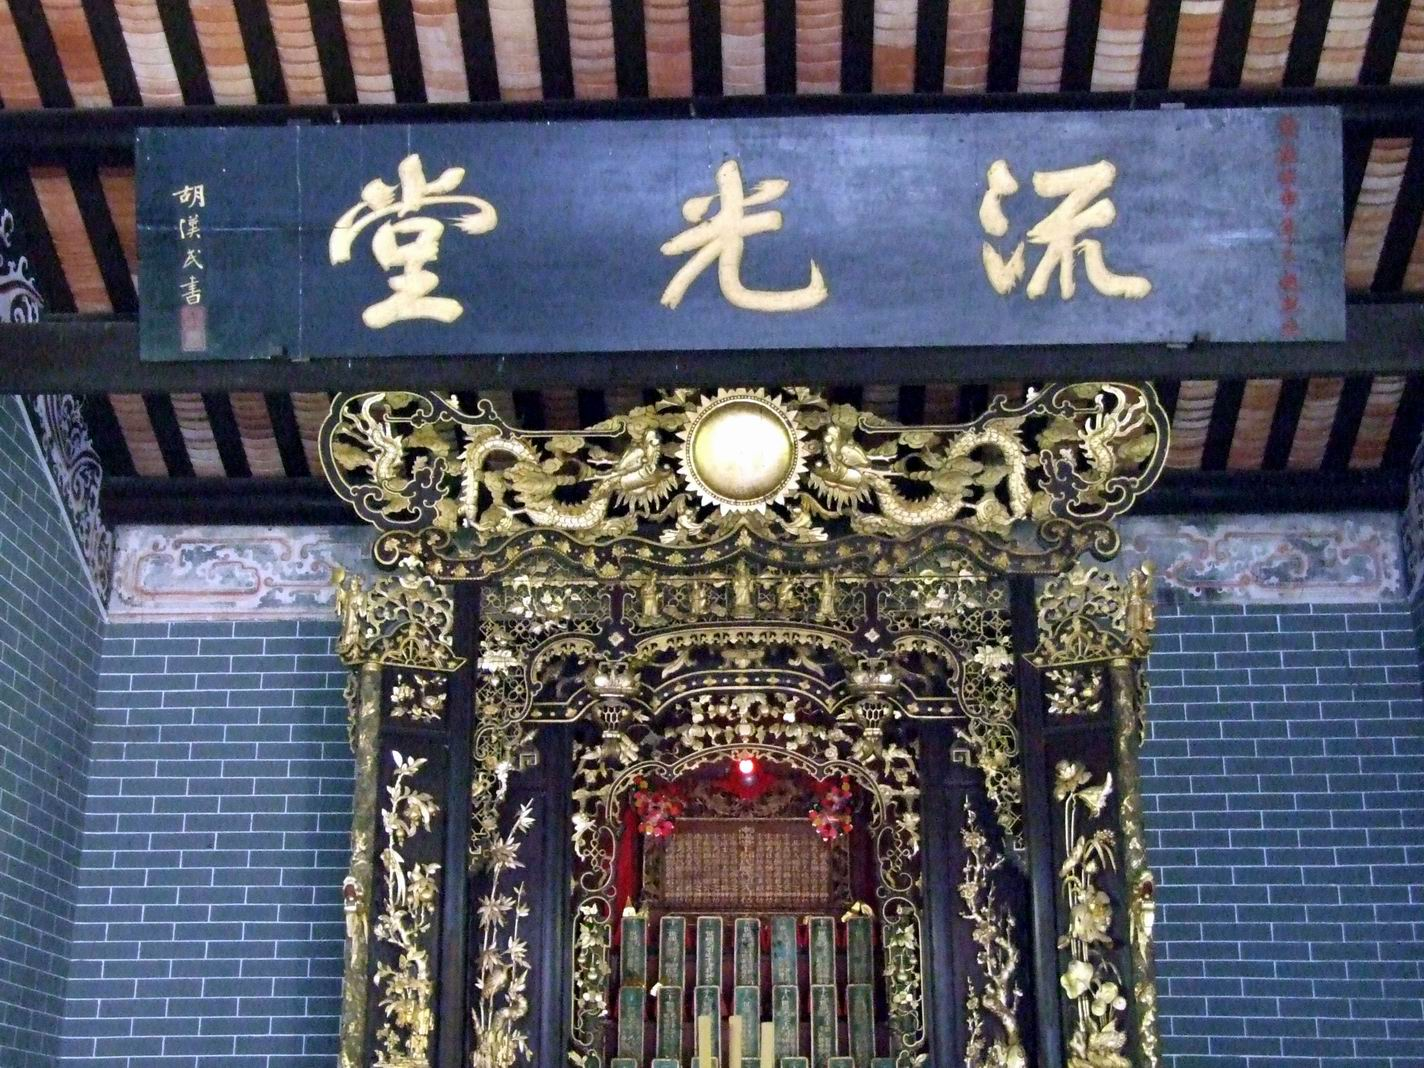
\includegraphics[scale=0.15]{./figs/KingLawKaShuk_Altar.jpg}
\end{center}
\end{frame}
{
  \setbeamercolor{background canvas}{bg=}
  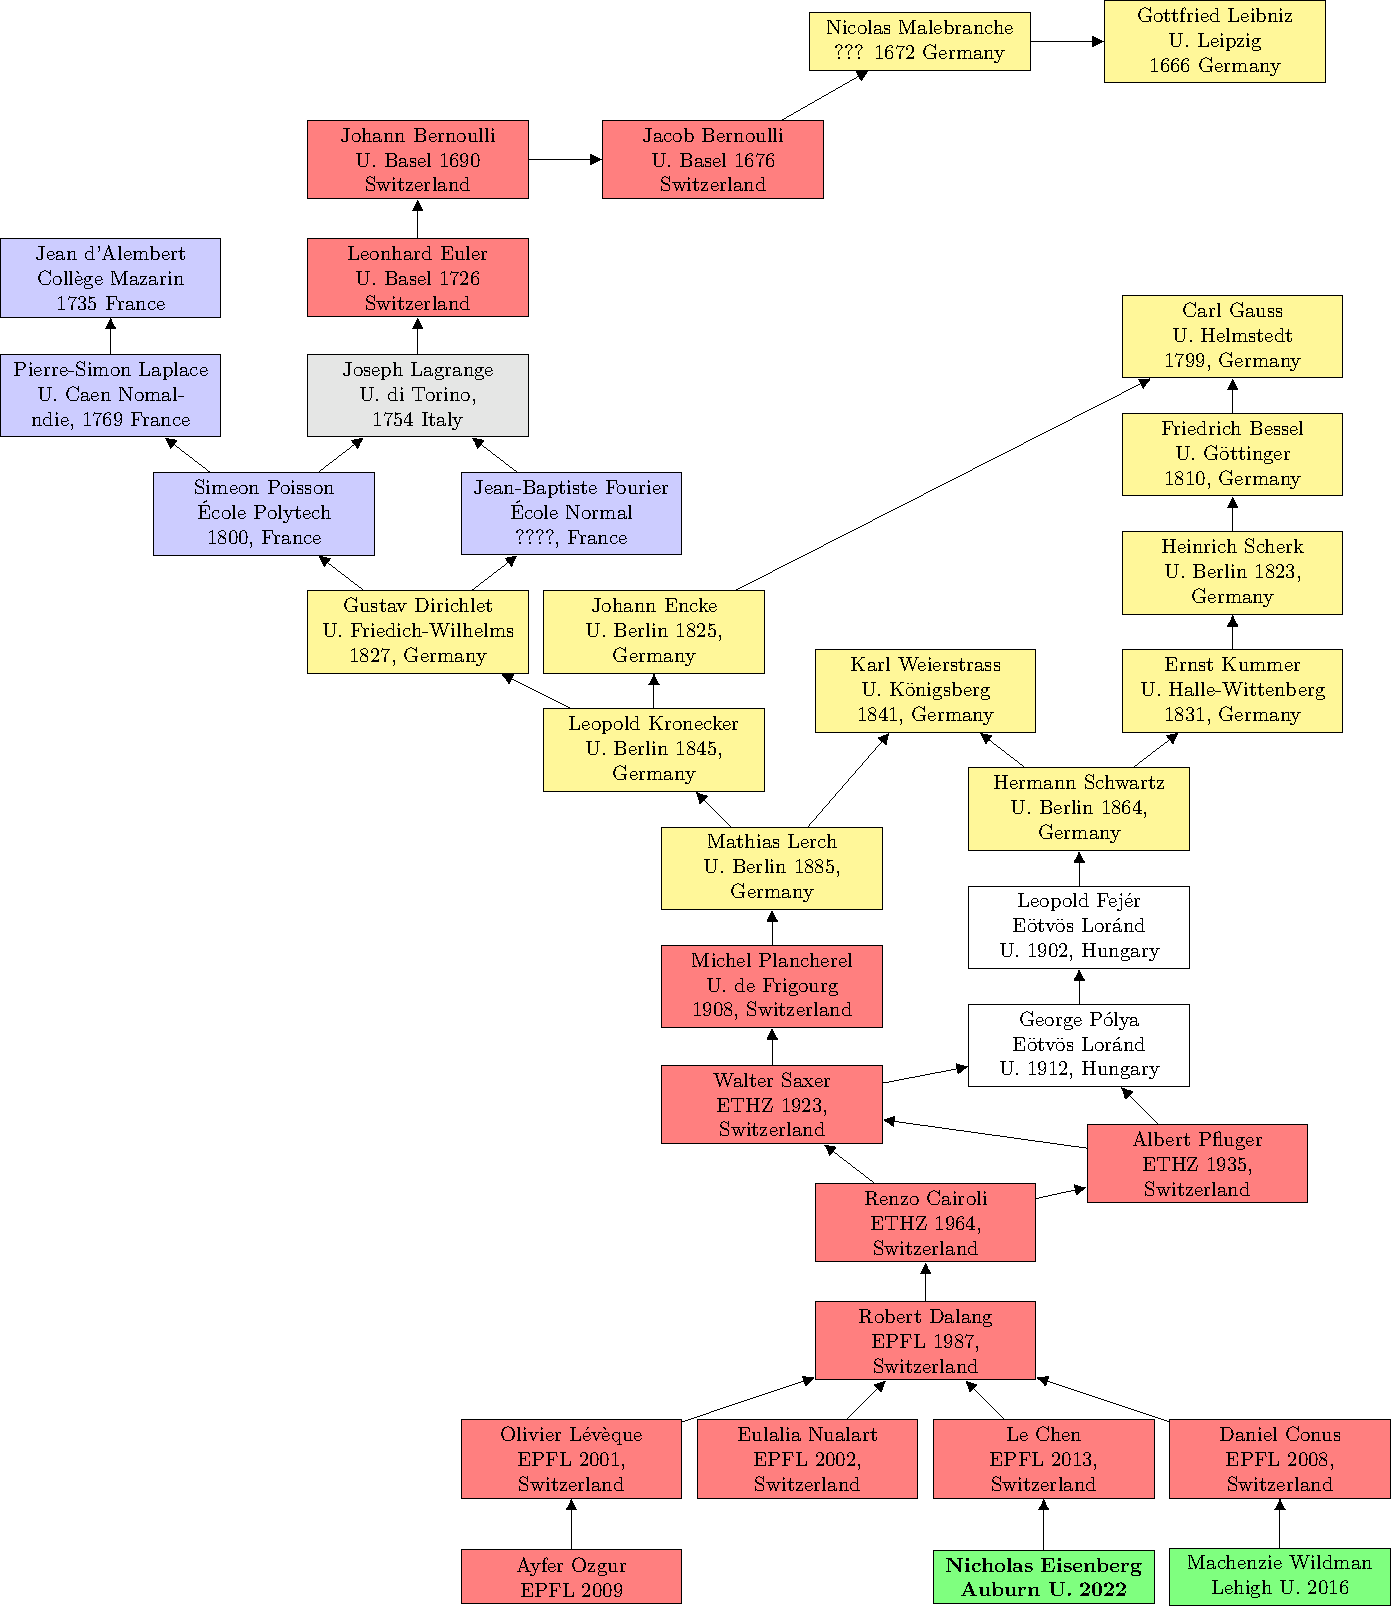
\includepdf[page=1]{../MathGenealogy.pdf}
 }
\begin{frame}[fragile] % Burn
\begin{center}
  \huge

  {\huge Dr. Eisenberg} \\
  \bigskip
  \bigskip

  is ``born" in the summer of 2022,\\

  \bigskip

  on the longest day of that year~!
\end{center}
\end{frame}
\end{document}
